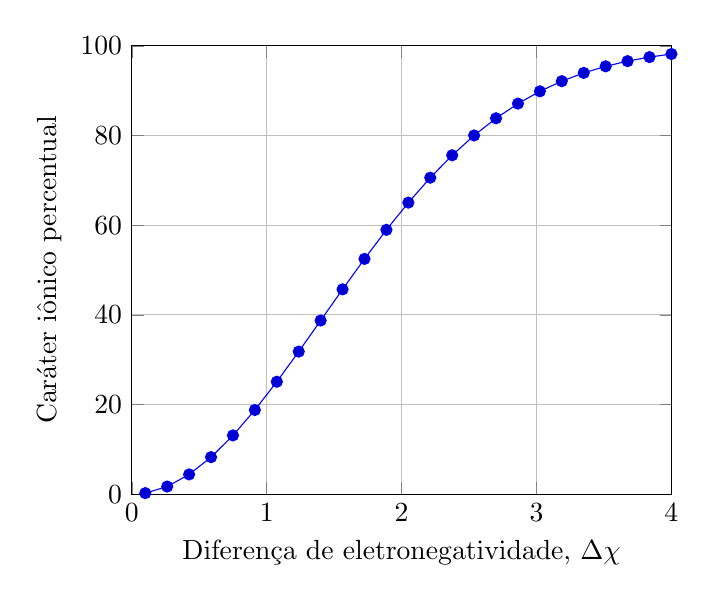
\begin{tikzpicture}
    \begin{axis}
        [
            grid = major,
            ylabel = {Caráter iônico percentual},
            xlabel = {Diferença de eletronegatividade, $\Delta \chi$},
            domain = 0.1:4,
            xmin = 0, xmax = 4,
            ymin = 0, ymax = 100,
        ]
    \addplot
        {
            100*(1 - exp(-x^2/4))
        };
    \end{axis}
\end{tikzpicture}

